\documentclass[12pt]{article} 
\usepackage{enumerate,geometry,fancyheadings,float,shortcuts,amsmath,lastpage,ifpdf,paunits,multicol}
\geometry{letterpaper,headsep=5mm,head=5mm,hmargin={25mm,20mm},bottom=10mm,top=10mm}

\ifpdf
    \usepackage[pdftex]{graphicx} 
    \usepackage{hyperref}    \pdfcompresslevel=0
    \DeclareGraphicsExtensions{.pdf,.jpg,.mps,.png}
\else
    \usepackage{hyperref}
    \usepackage[dvips]{graphicx}
    \DeclareGraphicsRule{.eps.gz}{eps}{.eps.bb}{`gzip -d #1}
    \DeclareGraphicsExtensions{.eps,.eps.gz}
\fi

\pagestyle{fancy} 
\lhead{Atsc. 405}
\chead{final}
\rhead{sample questions: page~\thepage/\pageref{LastPage}}
\lfoot{}
\cfoot{}
\rfoot{}
\begin{document}

\noindent

\begin{enumerate}


\item Tephigrams/thermo

  \begin{itemize}
  \item Take the derivitive of the moist static energy and, using a tephigram
  to get $dr_s/dT$
  estimate the moist adiabatic lapse rate:  $dT/dz$ at a point.


  \end{itemize}



\item  Size distributions

\par

Describe in as much detail as you can how a thermal diffusion
chamber is used to measure an atmospheric aerosol number and mass
distribution $n(D)\ (\un{m^{-3}\,\mum^{-1}}),\ m(D)\
(\un{kg\,m^{-3}\,\mum^{-1}})$ for a mixture of amonium bisulphate and
sodium chloride aerosols.  What are the physical principals
behind the instrument?  What assumptions need to be made?  Which would
you trust more $n(D)$ or $m(D)$, and why?



\item  Free energy

  \begin{enumerate}
  \item Use equation (\ref{eq:dg}) to show that, for a closed system consisting of a
flat puddle of water in equilibrium with vapor at temperature T, $g_l = g_v$.
\item Consider another system at the same temperature in which the same amount of liquid is
  redistributed as droplets of radius 0.1 \mum.  Would this system have
  a lower or higher $g_v$ in equilibrium?  Why?
\item How would the introduction of sulphate aerosols into each of these drops
change the equilibrium value of $g_v$ and $g_l$?
  \end{enumerate}


\item Kelvin equation

Show using \ref{eq:G} is that for pure supersaturated water
the equilibrium droplet radius found by setting
$\frac{\partial E }{\partial r} = 0$ is unstable.


\item Show that the energy difference between a sheet of polluted
water with activity $a_w$ and vapor with partial pressure
$e$ is given by:

\begin{equation}
  \label{diff}
  g_l - g_v = -R_v T \mathrm{ln} \left ( \frac{e}{e_s(T) a_w} \right )
\end{equation}


\item Explain the physical reasons (i.e. talk in terms of molecules) why:

\begin{itemize}
\item Increasing the activity makes the difference less negative
\item Decreasing the vapor pressure makes the difference less negative
\end{itemize}

Why does a low value of the activity help droplets to form?


\item The figure below shows typical aerosol 
    number, surface area and volume distributions.
    \begin{enumerate}
    \item Derive an equation relating $d V/d\log D$ to $d  N/d\log D$.
    \item Explain how you would find the average radius of the
      aerosol  distribution using data from this figure.
    \end{enumerate}    

    \begin{figure}[H]
      \begin{center}
        \leavevmode
  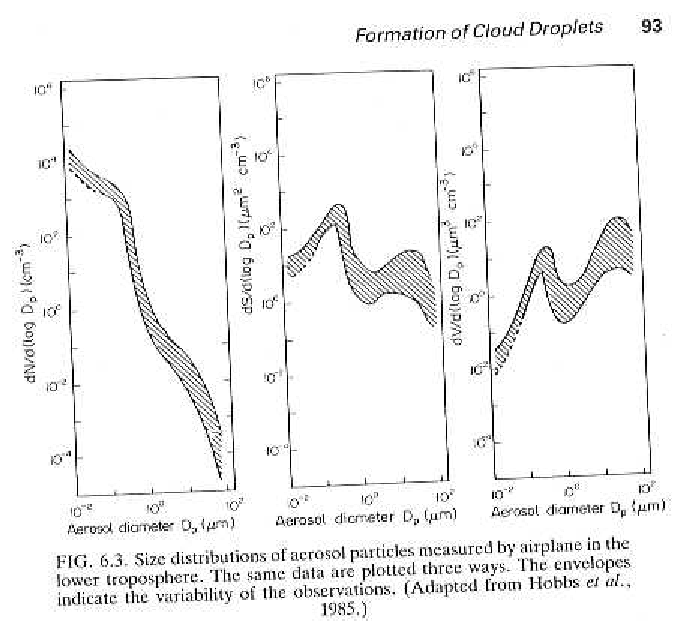
\includegraphics[width=6in]{aero}
        \label{fig:aer}
    \caption{$ $}
      \end{center}
    \end{figure}


\item Suppose a cloud chamber is filled with aerosols with masses
between $10^{-19} - 10^{-17}\ kg$.   The saturation S=$e/e_s$ in the
chamber is gradually increased from 0.9 (below $S_{crit}$ for all the
aerosols) to 1.1 (above $S_{crit}$ for all aerosols).  Pick two
aerosols with different masses and describe qualitatively (and using
graphs of their K\"ohler curves) what happens to them
(growth?, evaporation?, equilibrium?, non-equilbrium?)  as the
supersaturation is increased, and why.

\item A laser is used to measure the total number of water droplets
(with, say, radii bigger than 3 $\mu m$) in the
chamber at each saturation as we ramp up S.  Explain how this can be used to
get the mass size distribution (i.e. $m(D)$ where $m(D)dD$ is the dry
mass of the aerosols with diameters between D and D+dD) of the dry
aerosols?


\item For the cloud chamber shown in this picture:

\includegraphics{chamber}

Why is the vapor pressure $e$ a linear function of distance between
the plates?  (Hint:  what is the profile of $r_v$ between the top
and bottom?)

\item  Show using a Taylor's series expansion that the activity $a_w$ can be approximated as: 
  \begin{equation}
    \label{eq:aw}
    a_w = \frac{n_w}{n_s + n_w} \approx 1 - \frac{b}{r^3}
  \end{equation}
where b is given by the formula on page~\pageref{constants}



\item Consider the following figure:

\vspace{-1in}

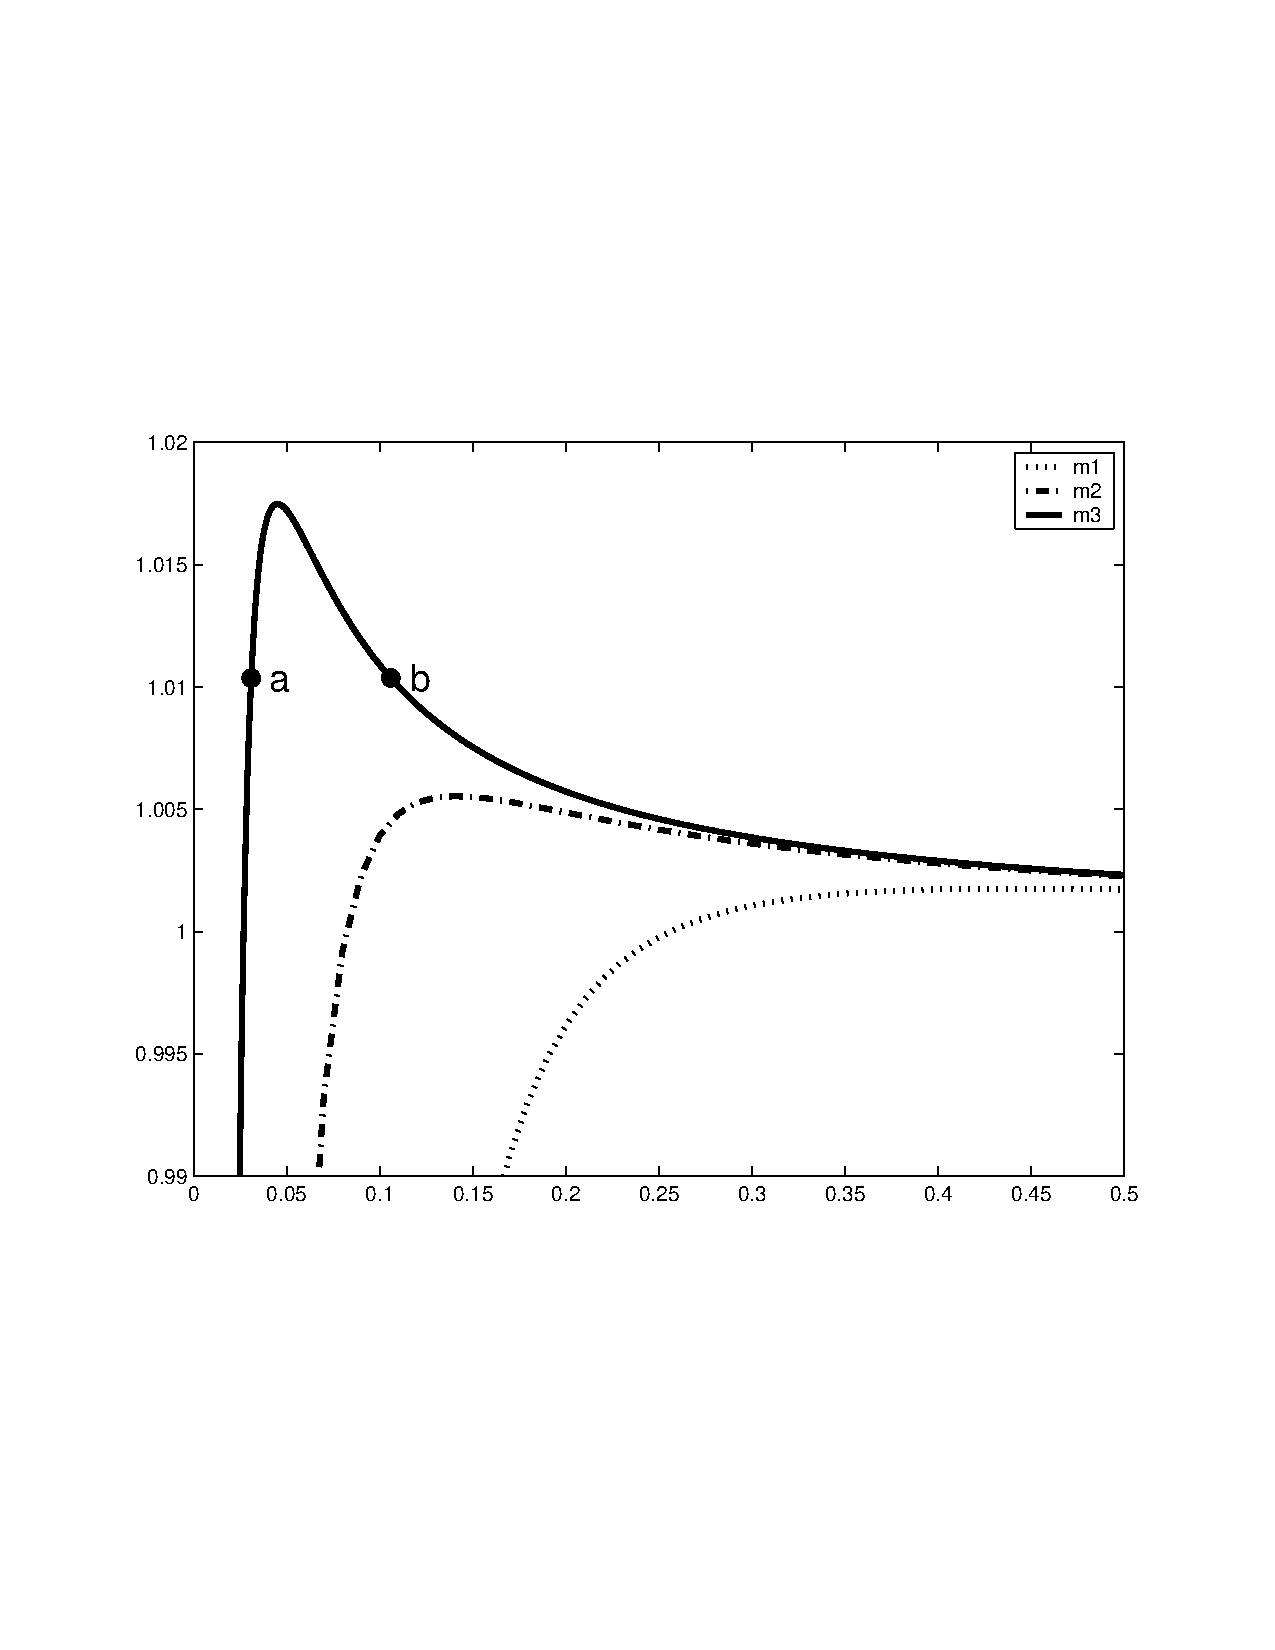
\includegraphics[width=0.8\textwidth]{finalfig}

\vspace{-1.5in}

  \begin{enumerate}
  \item  Which of the three aerosol masses $m_1$, $m_2$, $m_3$ is largest?  How do you know?
  \item Give a physical explanation (i.e.~argue in terms of the energies of vapor and liquid) why
       the equilibrium vapor pressure increases rapidly with radius near point a, and decreases
    with radius near point b.
  \end{enumerate}


\item   Starting with the expression for the Gibbs free energy:

\begin{equation}
  \label{gibbs}
  dg \leq - s dT + \alpha de
\end{equation}

Show that the energy difference between a flat sheet of pure
water and vapor with partial pressure
$e$ is given by:

\begin{equation}
  \label{diff1}
  g_l - g_v = -R_v T \mathrm{ln} \left ( \frac{e}{e_s(T)} \right )
\end{equation}

\item  For a mixture of liquid and vapor $G=m_v g_v + m_l g_l$.  
Use that fact to
show that $e=e_s(T)$ in equilibrium.  What assumptions have you made?

\item Suppose we have water vapor at a supersaturation of 5\% and a
  temperature of 280 K, and that $e_s(280)$ = 10 hPa.  
How much energy, in Joules, could the system
  release by condensing out a mass of water equivalent to a single
  0.01 \mum drop?  How does that compare to the surface energy
  required to build that drop?  Explain the significance of these
  numbers for the process of cloud formation in the atmosphere.


\item How is  (\ref{eq:cc}) related to the Clausius-Clapeyron equation?


\item What is droplet ``activation?''



\end{enumerate}



\textbf{CAPE}

\begin{enumerate}
\item[CA1]  How would you calculate the CAPE of a sounding given the
python thermodynamics library developed in this course?
\end{enumerate}

\textbf{Droplet growth}

\begin{enumerate}
\item[D1] Approximately how many seconds does it take to double the radius of
a 10 $\mu m$ drop exposed to a supersaturation of 1\%, at a temperature of
280 K? (Neglect Kelvin and Raoult effects).

\item[D2] What is steady about ``steady state'' droplet growth? Explain,
using appropriate equations for the droplet mass and the vapor density.

\item[D3] This figure  shows that if you quadruple the
updraft velocity of a parcel containing aerosols from a weak (0.5 \ms)
to strong (2 \ms), you: 1) increase the maximum supersaturation
of the parcel, 2) increase the droplet concentration, 3) decrease the average
drop size.  Use your knowledge of the droplet growth equation, aerosol
size distributions and the K\"ohler curve to explain 1-3.

    \begin{figure}[H]
      \begin{center}
        \leavevmode
  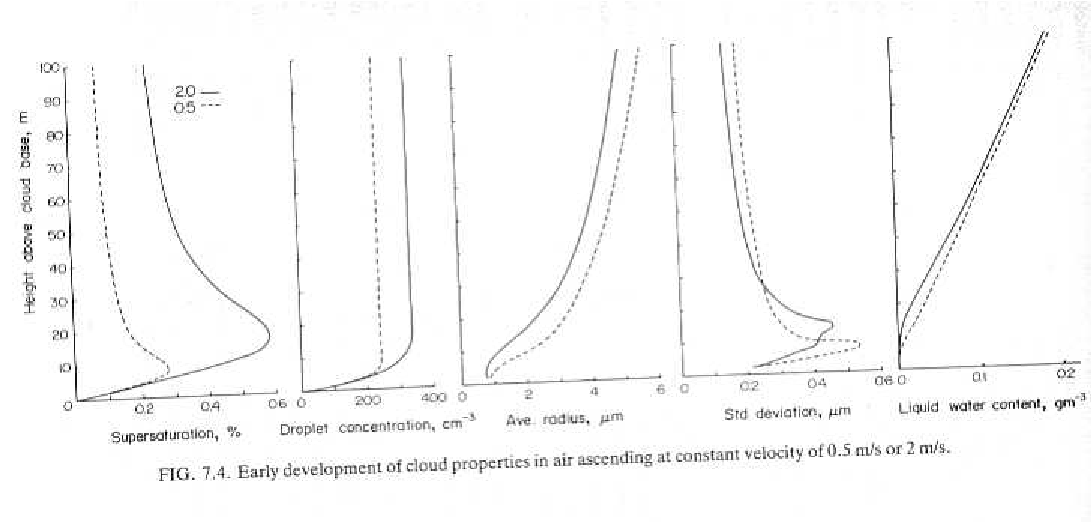
\includegraphics[width=6in]{supersat}
        \label{fig:supersat}
    \caption{$ $}
      \end{center}
    \end{figure}

\item[D4] Show using the droplet growth equation (and neglecting the Raoult and Kelvin
terms) that if the environmental supersaturation
remains fixed, the radial growth rate $dr/dt$ decreases with increasing $r$.
Why is this important?


\item[D5] Suppose you have $N=10^8\,m^{-3}$ aerosols, all the same size
  and composition with a critical saturation of S=1.005.  These
  aerosols are placed in an adiabatic updraft (vertical velocity=0.5
  $m\,s^{-1}$) with an initial saturation of S= 0.8 and a temperature
  of 280 K.  Explain in as much detail as possible how you could
  calculate the growth of these aerosols into cloud droplets as a
  function of time (assuming that you can calculate the change in a
  quantiy like mass
  $\Delta m$ during a time step $\Delta t$ via $\Delta m =
  \frac{dm}{dt} \Delta t$). Use the equations listed below and
  whatever other relations you think necessary.  Assume that you also
  know the shape of their K\"ohler curve, and don't forget to discuss
  how you would start the calculation.

\item[D6] Explain how, and why, the supersaturation over the drop surface and
the drop growth rate would change for each of the following:


\begin{itemize}
\item A decrease in the surface tension, $\sigma$
\item Radiative cooling of the drop.
\item An increase in the latent heat of vaporization
\item A increase in the number of sulphate ions on the drop surface
\end{itemize}



\item[D7] Show  with the help of a figure why:

  \begin{equation}
    \label{eq:flux}
    \frac{\partial \rho_v}{\partial t} =  D  \nabla^2 \rho_v
  \end{equation}

\end{enumerate}

\noindent
\textbf{Coalescense:}

\begin{enumerate}

\item[C1] 

  \begin{enumerate}
  \item Make a sketch of the the collision efficiency E as a function
    of ratio of small droplet radius to collector radius for a given
    collector drop.  Why does E exceed 1 for large values of the
    ratio?
  \item What is the difference between stochastic and continuous
    collection? Explain how stochastic collection can account for the
    observation rapid development of precipitation in warm clouds.
  \item Why are the details of the coalescence process less important
    in clouds with ice?
  \end{enumerate}


\item[C2] Suppose you know that cloud drops have a size distribution given
  by 
  \begin{equation}
    \label{marshall}
    N(r)=N_0 \exp (- \chi r)
  \end{equation}
\noindent
where $N(r)$ ($\mathrm m^{-3}$) is the number of drops with radius $>
r$ (for radii $50\ \mathrm{\mu m} < r < 200\ \mathrm{\mu m}$ ) and $N_0$
and $\chi$ are constants.  Suppose also that the drop fall speed
$v(r)\ (\mathrm{m\,s^{-1}})$ 
depends on linearly on radius:
\begin{equation}
  \label{fallspeed}
  v(r)=Jr
\end{equation}

Derive equations (with unit conversions if necessary) for:

\begin{enumerate}
\item The liquid water content ($\mathrm{kg\,m^{-3}}$)
\item The precipitation rate ($\mathrm{mm\,hr^{-1}}$)
\end{enumerate}


\item[C3] Show that a simple model of the growth of rain drops
    (\ref{eq:collec}) predicts exponential growth of drop radius with
    time.  How large is the time constant for this growth? (assume a
    droplet population with $r_l = 0.3\ g\,m^{-3}$ and state any other
    assumptions you make).  What processes need to be added to
    (\ref{eq:collec}) to make the description of rain formation more
    accurate? Explain.



  \item[C4]  Do Wallace and Hobbs 6.24

\end{enumerate}

\textbf{Python}

\begin{enumerate}
\item[M1]  Suppose you put 1 kg of liquid water in a sealed 5 liter container 
at 280 K.  Describe qualitatively how you would write a python
script to  accurately determine the mass of vapor and liquid at
equilibrium.  (Hint:  think about using the fzero rootfinder, and
conservation of mass and volume).


\item[M2] Write python function that would evaluate derivatives needed to
find  $r_l$ as with height assuming saturation, constant $\theta_e$,
conservation of water in a hydrostatic atmosphere.


\end{enumerate}

\textbf{Thermo}

\begin{enumerate}
\item[T1]  We've seen equations for $\theta$, $h$, $\theta_e$, $\theta_{es}$, $s_{me}$, $G$,
and $S$.  For each of these pick a situation in which it is the variable of choice to
describe a system or process, and explain what it is about the variable that makes it
particularly well suited to the problem.


\item[T2]  We know that a plume of dry air is continually mixing in air from its environment,
yet a balloon sounding will show that its temperature/pressure profile is very close
to adiabatic.  How is this possible?

\item[T3]  Two pots of water sit side by side.  One is completely
insulated, the other is free to exchange energy with an
infinite reservoir.  You put a liter of liquid water in each and
seal them.   Describe qualitatively how you would find the
equilibrium temperature and vapor pressure in each pot using
(you could use python), and why they will be different, even if
the liquid water is starts at the same temperature in each.


\item[T4] Find the entropy of a kg of vapor
referenced to liquid water  at temperature $T_p$ and pressure $e_s(T_p)$ in
contact with thermal reservoir.  Show that reversibly moving 1 kg
of water from liquid to vapor while keeping the temperature
and presure constant requires that the reservoir supply
the vapor + liquid system with entropy $S=\frac{ l_v}{T}$



\end{enumerate}





\newpage
\begin{center}
  \textbf{Equation sheet}
\end{center}

\begin{multicols}{2}

  \begin{equation}
\label{eq:first}
du = q\,dt - w\,dt = q\,dt - p\,d\alpha
  \end{equation}

\begin{equation}
e = \rho_v\, R_v\, T
\end{equation}

\begin{equation}
p = \rho\, R_d\, T_v
\end{equation}


\begin{equation}
w \,dt = p\,d\alpha
\end{equation}

\begin{equation}
h = u + p \,\alpha
\end{equation}

\begin{equation}
  \label{eq:tv}
  T_v = T(1 + 0.608 r_v - r_l)
\end{equation}

\begin{equation}
  \label{eq:wv}
  r_v = \rho_s/\rho_d = \epsilon \frac{e_s}{p - e_s}
\end{equation}

\begin{equation}
dh = c_{px}\, dT\ \mathrm(dry\ air\ or\ liquid)
\end{equation}

\begin{equation}
dh = c_p\, dT\ + l_v\,dr_v\ \mathrm(air/water\ mixture)
\end{equation}


\begin{equation}
dh = T\,ds + \alpha\,dp\ \mathrm(reversible)
\end{equation}

\begin{equation}
ds = c_p \frac{d\theta}{\theta} = c_p \frac{dT}{T} - R_d \frac{dp}{p}
\end{equation}

\begin{equation}
  \label{eq:ds}
  ds \geq \frac{q\,dt}{T}
\end{equation}

\begin{equation}
l_v = h_v - h_l
\end{equation}


\begin{equation}
dp = - \rho\,g\,dz
\end{equation}


\begin{equation}
\label{eq:moist}
  dh_m = c_p\,dT + l_v\,dr_v + g\,dz
\end{equation}

\begin{equation}
\label{eq:theta}
  ds = c_p \frac{d\theta_e}{\theta_e} = c_p \frac{d\theta}{\theta} + \frac{l_v\,dr_s}{T}
\end{equation}

\begin{equation}
  ds = c_p \frac{d\theta_l}{\theta_l} = c_p \frac{d\theta}{\theta} - \frac{l_v\,dr_l}{T}
\end{equation}

\begin{multline}
  buoyancy = g \frac{\rho_e - \rho_p}{\rho_e} \approx g \frac{T_{vp} - T_{ve}}{T_{ve}} \\
 = g \frac{T_v^\prime}{\overline{T_v}} \approx g \frac{\theta^\prime}{\overline{\theta}}
\end{multline}

\begin{equation}
  \label{eq:bv1}
  z^\prime(t) = z^\prime (0) \cos N t
\end{equation}

\begin{equation}
  \label{eq:bv2}
  N^2 = \frac{g}{T} ( \Gamma_d - \Gamma )
\end{equation}


\begin{equation}
  \label{eq:wdiff}
  d r_v = \frac{r_v}{p-e} \left ( \frac{p}{e} de - dp \right )
\end{equation}

\begin{eqnarray}
  \label{eq:taylor}
  f(x)  &=& f(x_0) + f^\prime(x_0)(x - x_0) \nonumber\\ 
        &+&  \frac{f^{\prime\prime}(x_0)}{2}(x-x_0)^2 +  \ldots
\end{eqnarray}

\begin{gather}
\label{eq:cc}
  l_v = T (s_v^* - s_l)
\end{gather}

\begin{gather}
  \frac{de_s }{dT} = \frac{l_v e_s}{R_v T^2} 
\end{gather}


\begin{subequations}
  \begin{eqnarray}
  h_l = c_l (T - T_p) \\
 h_v = l_{v0} + c_{pv} ( T - T_p) \\
s_d = c_{pd} \log T - R_d \log p_d\\
 s_l = c_l \ln \frac{T }{T_p}  \\
 s_v = c_{pv} \ln \frac{T }{T_p} - R_v \frac{e }{e_{s0}} + \frac{l_{v0} }{T_p}  
\label{eq:sref}
  \end{eqnarray}
\end{subequations}


  \begin{equation}
  g = u + p\alpha - Ts = h - Ts
  \end{equation}

  \begin{equation}
    \label{eq:dg}
    dg \leq -s dT + \alpha dp
  \end{equation}


  \begin{equation}
    \label{eq:G}
    E = m_v g_v + m_l g_l + 4 \pi \sigma r^2
  \end{equation}

  \begin{equation}
    \label{eq:newint}
    \int_{a_w e_s}^e  d(g_l - g_v) \approx  - R_v T\ln \left (
      \frac{S}{a_w} \right )
  \end{equation}



\begin{multline}
  \label{equil}
  e_{\chi} = e_s(T)(n_w/(n_w + n_s))\exp(a/r) \\
  = e_s(T)(1 + \frac{a}{r} - \frac{b}{r^3})
\end{multline}

\begin{equation}
  \label{eq:sscrit}
  s_{crit}= 1 + \left ( \frac{4 a^3}{27 b} \right )^{1/2}
\end{equation}

\begin{equation}
  \label{eq:rcrit}
  r_{crit} = \left ( \frac{3b}{a} \right )^{1/2}
\end{equation}

\begin{equation}
  \label{eq:2ndb}
  c_p \frac{d\theta_e^\prime}{\theta_e^\prime} = 
          \frac{dm}{m} \frac{\Delta h_m}{T^\prime}
\end{equation}

\begin{equation}
  \label{eq:plume}
  \frac{1}{m} \frac{dm}{dt} = \lambda
\end{equation}

\begin{equation}
  \label{eq:water}
  \frac{dw_T^\prime}{dz} = (w - w_T^\prime) \hat{\lambda}
\end{equation}

\begin{equation}
  \label{eq:collec}
  \frac{dM}{dt} = \pi R^2 E (V(R) - V(r)) r_l
\end{equation}
where V(r) $\approx$ 0 and V(R) $\approx$ JR (with J=6000 $s^{-1}, R in \un{m}$)

\begin{equation}
  \label{eq:dropgrow}
  \frac{dm}{dt} = 4 \pi r D (\rho_{v \infty} - \rho_{v r})
\end{equation}



\label{constants}
\begin{tabular}{ll}
$a$ & $\frac{2 \sigma}{\rho_w R_v T}$  \\
$b$  &  $\frac{i m M_w}{(4/3)M_s \pi\rho}$ \\ 
$\sigma$ & 0.075 \un{J\,m^{-2}}\\
$\rho_w$ & 1000  $\un{kg\,m^{-3}}$ \\
$c_{pd}$ & 1006\ \un{J\,kg^{-1}\,K^{-1}}\\
$c_{pv}$ & 1870\ \un{J\,kg^{-1}\,K^{-1}}\\
$c_l$    & 4190\ \un{J\,kg^{-1}\,K^{-1}}\\
$D$      & 2.36 $\times 10^{-5}$ \un{m^2\,s^{-1}}\\
$R_d$    & 287\ \un{J\,kg^{-1}\,K^{-1}}\\
$R_v$    & 461\ \un{J\,kg^{-1}\,K^{-1}}\\
$k$      & 1.381 $\times 10^{-23}$\ \un{J\,K^{-1}\,molecule^{-1}}\\
$l_{v0}$    & 2.5 $\times 10^6 $\ \un{J\,kg}\mbox{ at 0 deg C}
$K \approx 2.5 \times 10^{-2}$ \un{J\,m^{-1}\,s^{-1} K^{-1}}
$D \approx 2.4 \times 10^{-5}$ \un{m^{2}\,s^{-1}}
\end{tabular}

\end{multicols}


\end{document}


%%% Local Variables:
%%% mode: latex
%%% TeX-master: t
%%% End:
